\chapter{Introduction}
\label{ch:Intro}
\noindent{\textbf{\huge W}}e are currently living in the \textit{information age}, owing to the technological advances that enabled us to gather and analyze a lot of data. This explosion of data gave rise to the digital companies that strive to provide their clients a digital alternative to almost every aspect of their lives. We enjoy the luxury of these digital options ranging from virtual meetings to online shopping and from digital banking to automated medical diagnosis and fitness trackers. Various devices that support these technologies keep generating a lot of raw data that can be turned into usable knowledge. The knowledge, thus obtained, is the key for digital companies to provide their clients with a better experience in virtual or real life. Hence, the need to transform this data into usable knowledge increases.

Analysis of such a vast amount of data calls for algorithms that produce results in a very short time using less memory and can improve themselves by including newer data and getting rid of obsolete data. This thesis aims to fulfill this need in part by introducing four multi-view methods in the supervised learning domain. These methods are based on discriminant analysis and produce the same or even better results with significantly less time and memory requirements than the traditional machine learning algorithms. Multi-view learning, 2D methods, and incremental learning paradigms form the basis of the proposed methods. In this chapter, we look at the features of these paradigms that provide motivation and help in designing the methods presented in this thesis.







\subsubsection*{Multi-view Learning}
\label{ssubs:Intro_Mv}
Data acquired by different sources related by a common latent aspect is known as multi-view data. A view of an object is defined as a set of features that store information about a certain aspect of that object. The data samples within a view are assumed to be independent and identically distributed (IID). Multiple views of an object provide information about multiple aspects of the same object. The views of data are generated- (i) by observing the object using a single type of sensor from multiple perspectives, or (ii) by using multiple sensors of different types, or (iii) by obtaining independent sets of features from existing views. Fig. \ref{fig:Intro_MvData} shows examples of each of these three cases. Fig. \ref{fig:Intro_MvDataEx1} presents an example of case-(i) of multi-view data where each view is captured by a similar instrument, here- a camera. Each view has the same number of dimensions. All the views complement each other by capturing the same person from different angles. Another example of case-(i) is \cite{ChingovskaEAM16}, where a photograph of a person captured in the visual spectrum is one view, and a photograph of the same person captured in the infra-red spectrum is another view. Here, each view is a photograph, so their features are comparable. Both the views complement each other by capturing the same person in a different spectrum. Multiple views in fig. \ref{fig:Intro_MvDataEx2} represent case-(ii) as they are obtained from different sensors belonging to different domains, namely- audio, image, and text. As these views have different representations and features, they are not directly comparable in their original form. A similar example of case-(ii) is \cite{deSaB98}, which has a multi-view dataset for speech recognition with speech signals as one view and patterns of lip motion as another view. These views cannot be compared without transforming them into features that share a common subspace. Fig. \ref{fig:Intro_MvDataEx3} shows an example of case-(iii). The first view is a photograph of a person captured using a color camera. View-2 and view-3 are obtained from the first view by performing pixel average and edge detection operations, respectively. These views are also not directly comparable in their original form as they have different representations.



\begin{figure}[t]
\centering
  \begin{subfigure}{0.96\textwidth}
	\centering
    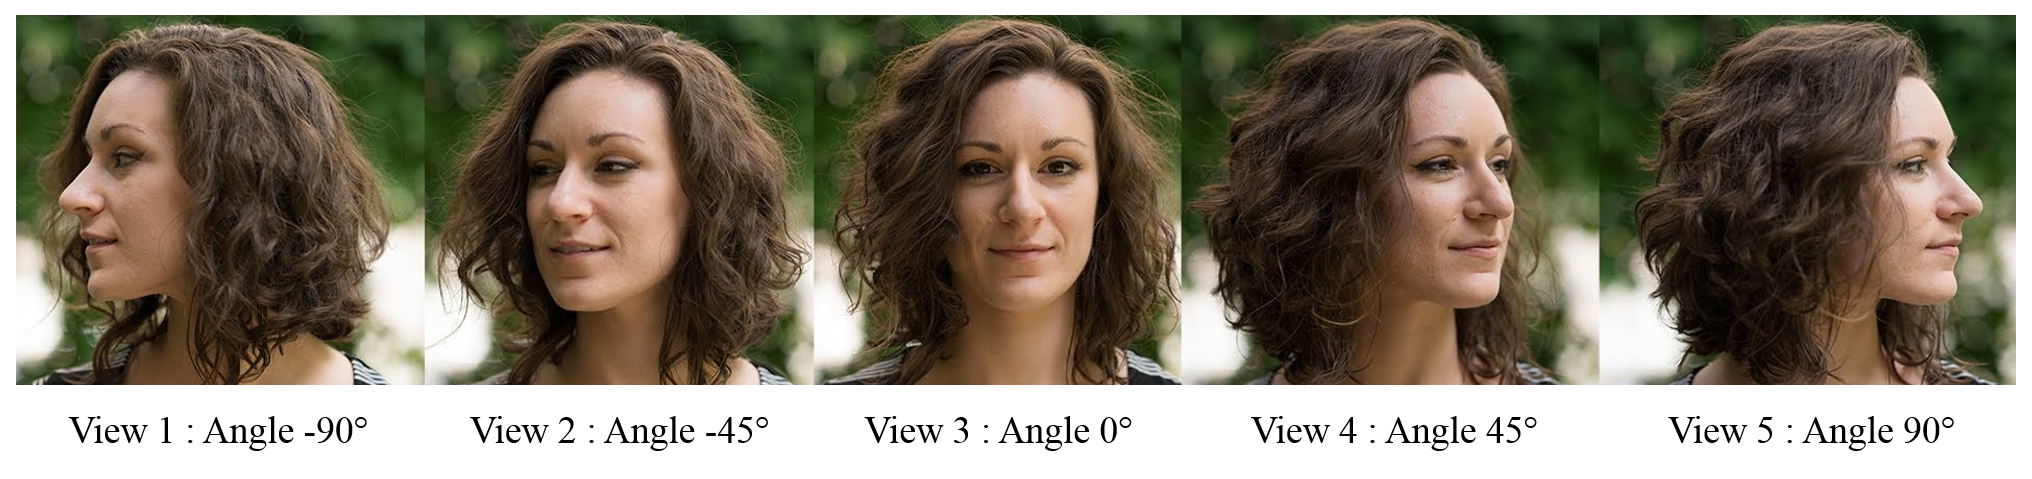
\includegraphics[width=\textwidth]{Figures/Introduction/Fig1a.png}
    \caption{Views obtained from a single sensor.}
    \label{fig:Intro_MvDataEx1}
  \end{subfigure}
  
  \begin{subfigure}{0.96\textwidth}
	\centering
    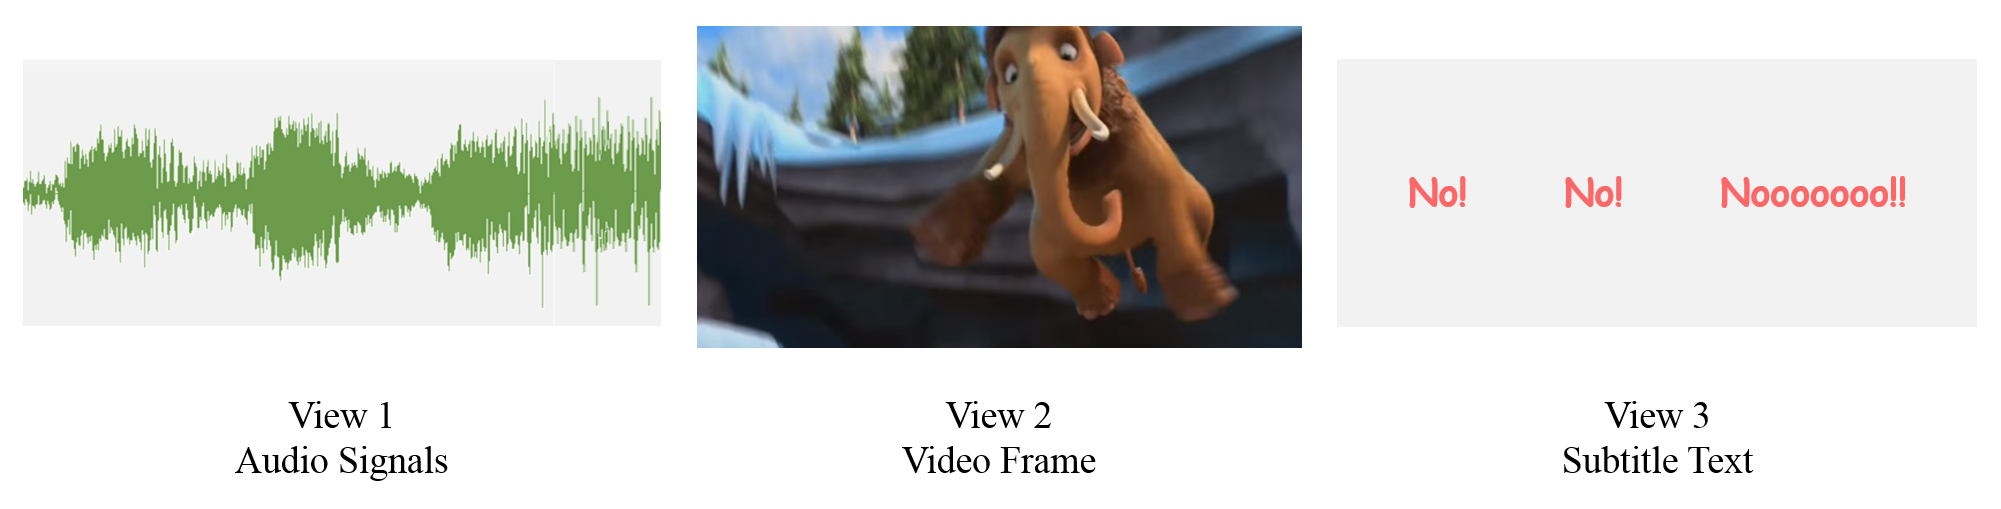
\includegraphics[width=\textwidth]{Figures/Introduction/Fig1b.png}
    \caption{Views obtained from different sensors.}
    \label{fig:Intro_MvDataEx2}
  \end{subfigure}
  
  \begin{subfigure}{0.96\textwidth}
	\centering
    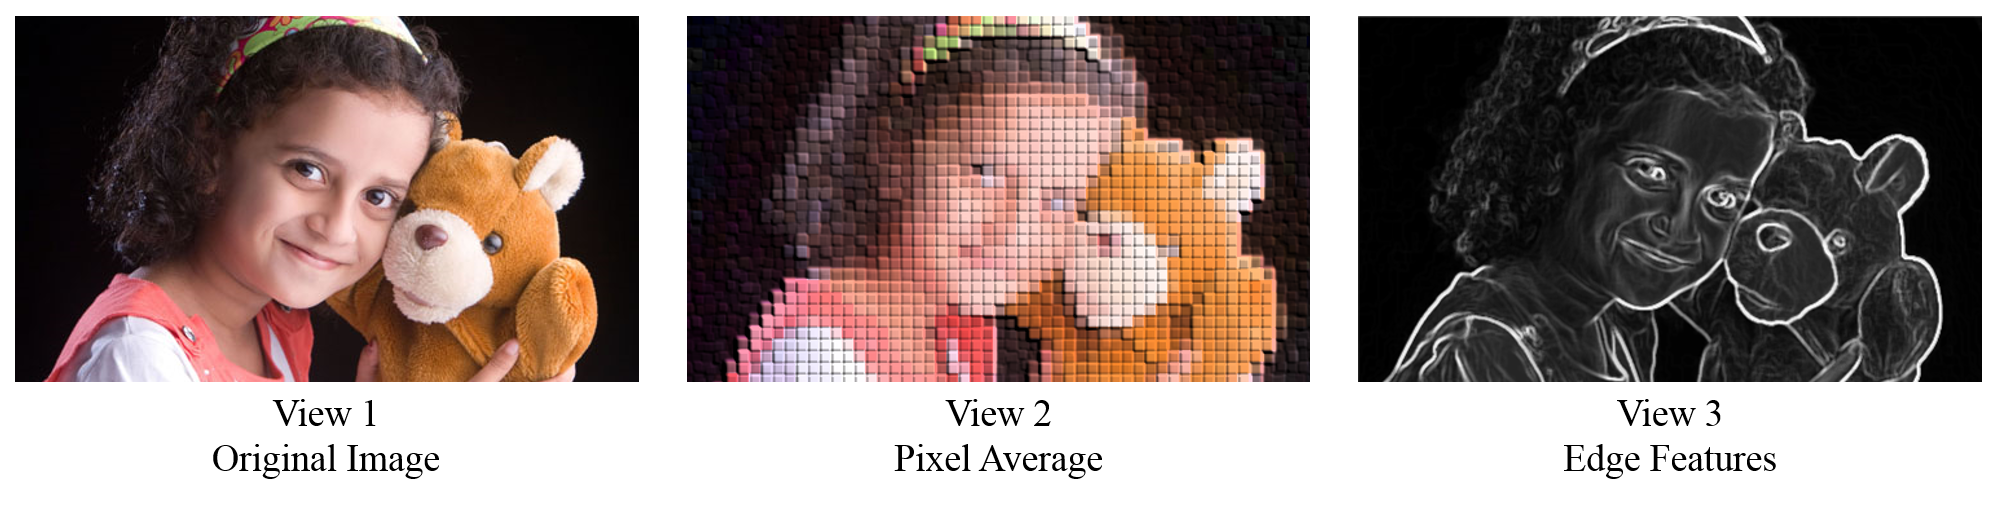
\includegraphics[width=\textwidth]{Figures/Introduction/Fig1c.png}
    \caption{Views derived from an existing view.}
    \label{fig:Intro_MvDataEx3}
  \end{subfigure}
\caption{Examples of multi-view data.}
\label{fig:Intro_MvData}
\end{figure}


Traditional machine learning used only one view of the underlying objects. The use of multiple views improves the performance of learned models because each view contributes some information about the underlying objects \cite{ZhaoXXS17, Sun13}. Fig. \ref{fig:Intro_Mv} shows an example that highlights the advantage of

\begin{figure}[t]
\centering
  \begin{subfigure}{\textwidth}
	\centering
    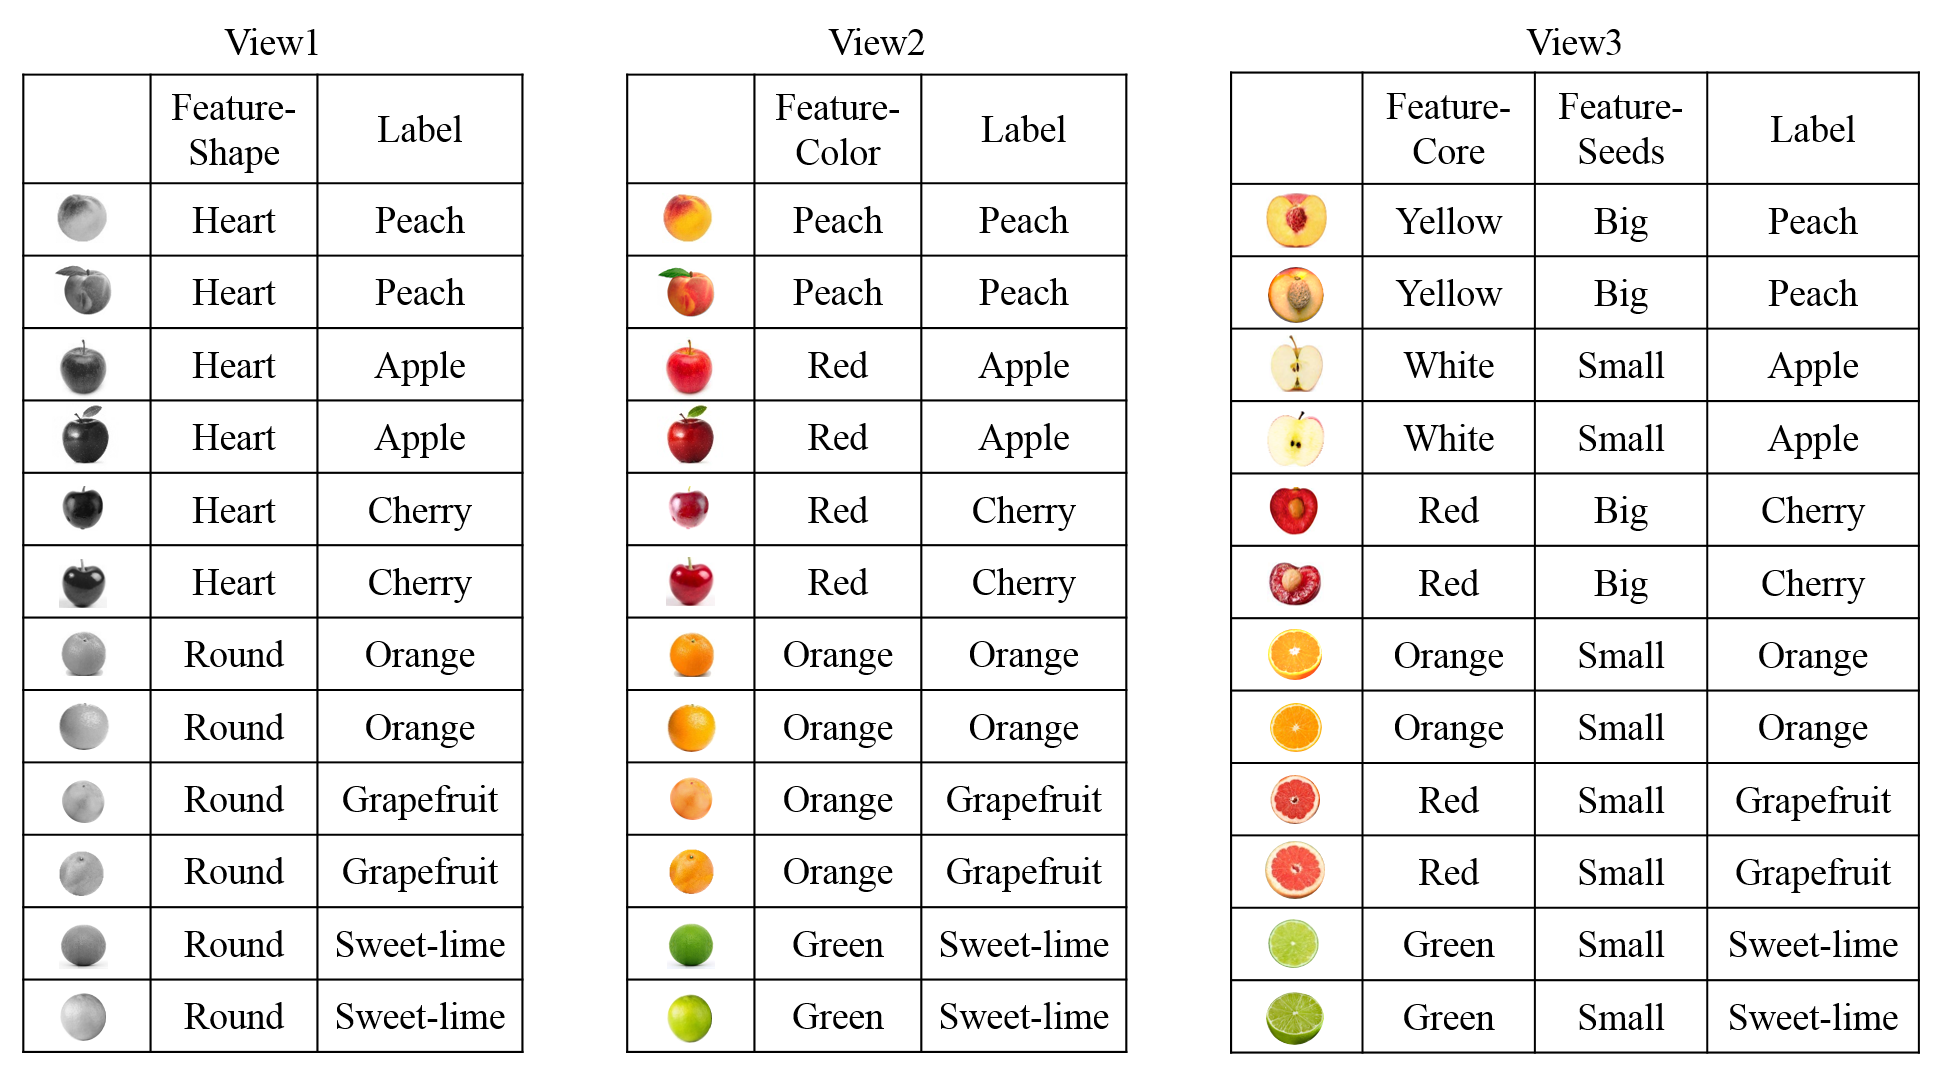
\includegraphics[width=\textwidth]{Figures/Introduction/Fig2.png}
    \caption{Training dataset that has three views}
    \label{fig:Intro_MvTrain}
  \end{subfigure}
  
  \begin{subfigure}{\textwidth}
	\centering
    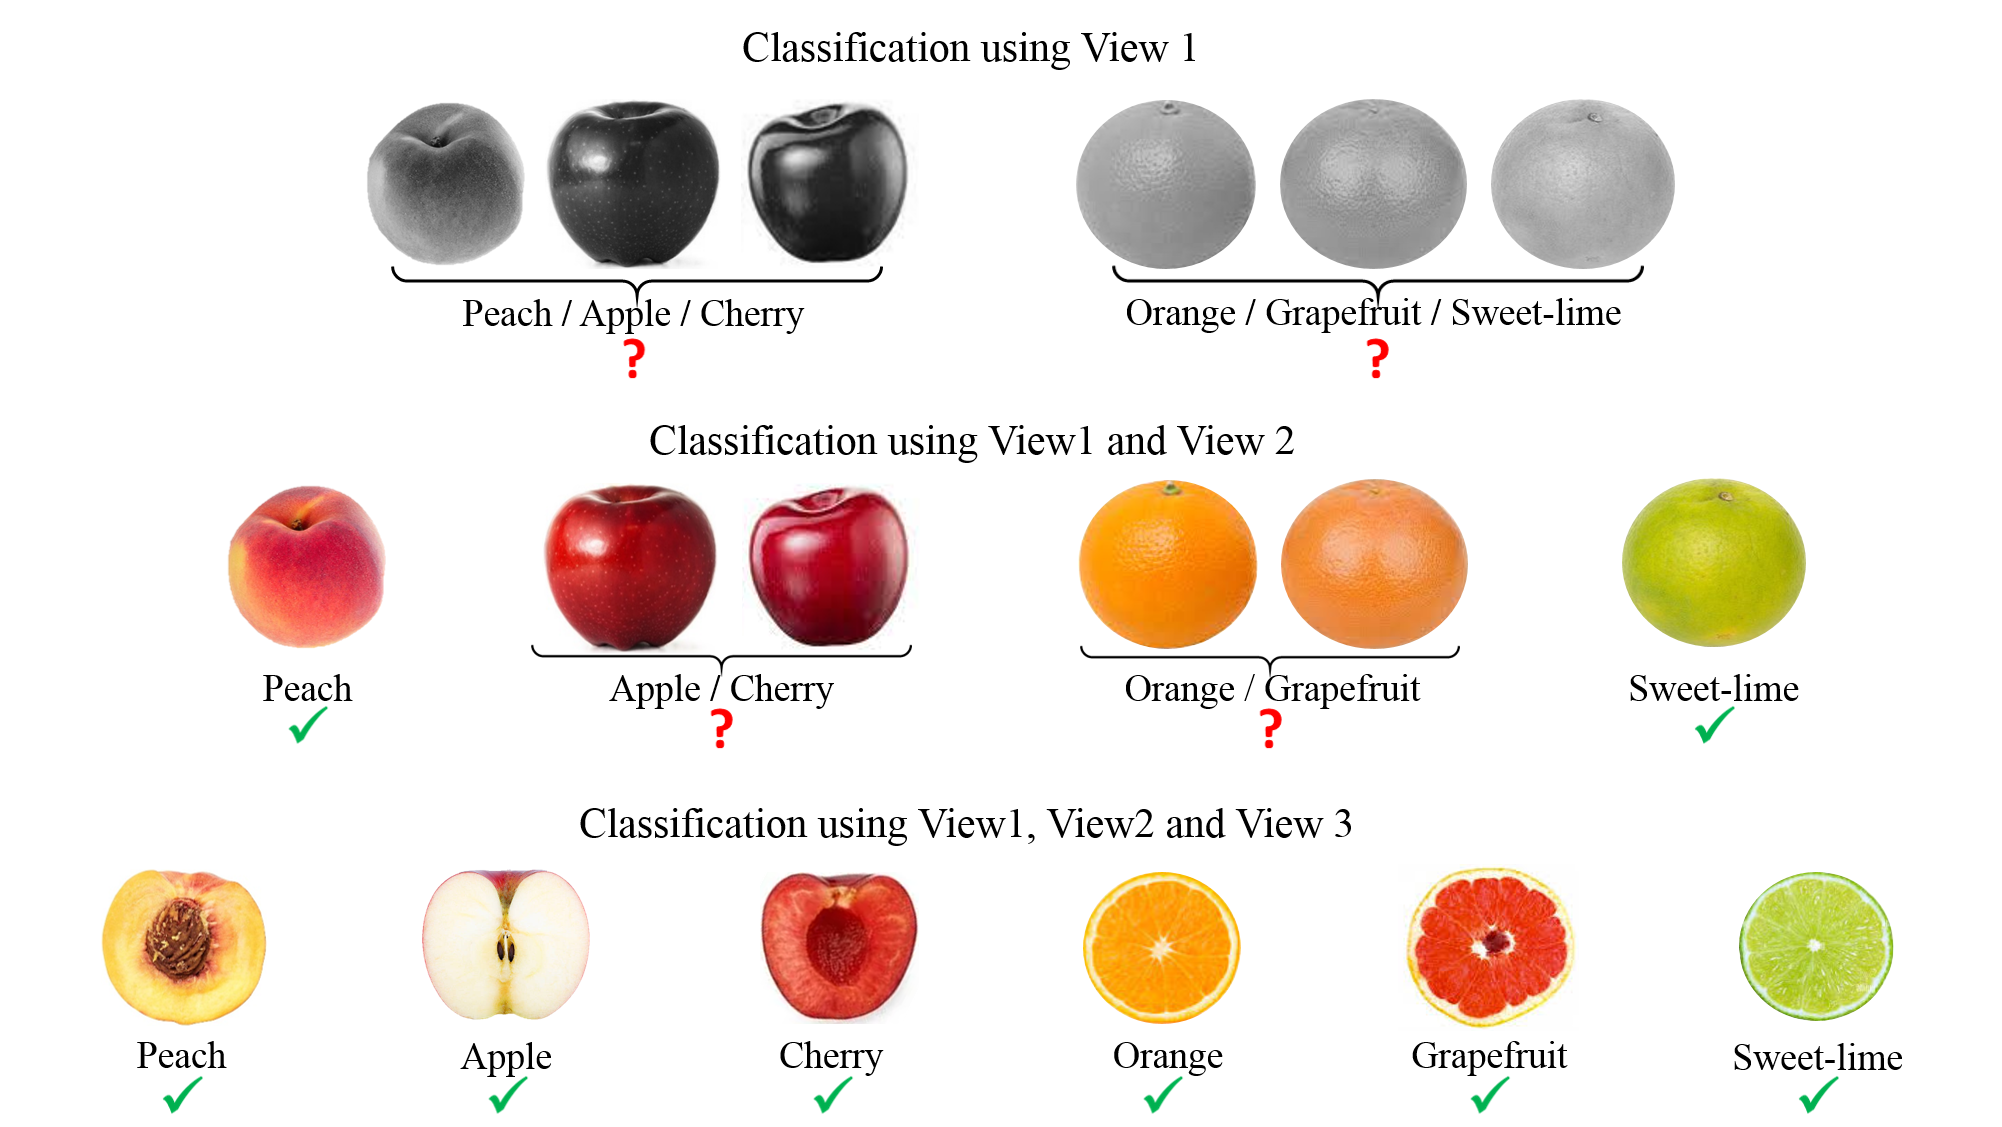
\includegraphics[width=\textwidth]{Figures/Introduction/Fig3.png}
    \caption{Classification performance on test set with gradually increasing views}
    \label{fig:Intro_MvTest}
  \end{subfigure}
\caption{An example to demonstrate the advantages of having multiple views. As the number of views increases, each view adds new complementary information. The learning algorithm leverages this information to improve its performance on each test data sample.}
\label{fig:Intro_Mv}
\end{figure}

\clearpage

\noindent
using multiple views of data. Here, we see a training dataset with three views- the shape of each fruit is one view, second is the color of a fruit, and the third one is the cross-section of each fruit. Three things to note here are- (i) Each view contains the features of every fruit in the training dataset, (ii) all views agree on the label of each fruit, (iii) Each view may have a different number of features in it. These three are the fundamental assumptions of multi-view learning. Given this dataset of fruits, the task is to learn to classify fruits in the test dataset. We see in Fig. \ref{fig:Intro_MvTest}, a model trained only on the first view has learned to distinguish between a heart-shaped and a round-shaped fruit, but it cannot distinguish between the fruits of the same shape as there are not enough features in that view that can teach the model to do so. We see three heart-shaped fruits and three round-shaped fruits in the test data. The information obtained from this view gives our model the ability to predict any label from (`peach', `apple', `cherry') for group-I and any label from (`orange', `grapefruit', `sweet-lime') for group-II. However, if we add a second view that describes the color of fruit and train a model on both the views, this model can see the facts that were not accessible using only the first view. Now, it can separate peach-colored `peach' from group-I and green-colored `sweet-lime' from group-II. However, it cannot distinguish between red-colored `apple' and `cherry', or orange-colored `orange' and `grapefruit'. When the third view that describes the pulp's color is added, each test sample can be labeled correctly because this view has more discriminatory information than the previous ones. This example demonstrates the benefit of using multiple views of the data that provide more object features that complement each other.

Due to their complementary nature, multiple views provide distinct information about the data, which is leveraged by the learning algorithms \cite{ZhaoXXS17, Sun13}. Hence, multi-view learning has been gaining attention in the recent past. Several multi-view algorithms have been developed over the years in different machine learning paradigms, such as supervised \cite{KanSZLC16,SunXY15,SharmaKDJ12,LiZLZ19}, semi-supervised \cite{ChaoS19,SunJ11}, active \cite{YuKRR11,SunH10}, unsupervised \cite{KumarD11,HouthuysLS18,KumarRD11} and transfer learning \cite{ChenWB11,XuS11}. These efforts demonstrate improvements in the performance of the algorithms due to the use of multiple views.

Multi-view data is used in various ways in different paradigms. Supervised methods use labeled data to train a model, and in multi-view learning, all views of an object in the training dataset agree with each other on its label. We can see the object-label pair as an input-output pair on which the model trains and, based on this training, produces output for the test objects. In the semi-supervised or active learning domain, labeled data is scarce, and the model has fewer data samples to train itself. Though the views agree on the labels of training data samples, due to the scarcity of ideal object-label pairs, they may produce different labels for test data samples. These conditions are often leveraged to expand the pool of labeled datasets by querying the labels of such data samples. Co-training\cite{BlumM98} and methods based on it \cite{NigamG00, SunJ11} train separate models on different views and use these models alternately to label a few data samples that were labeled by other models. Then, the data samples whose labels were most agreed upon are included in the training set to improve the models further. The views of data can even be thought of as being \textit{weak} or \textit{strong}. In the above example (Fig. \ref{fig:Intro_Mv}), we see that view-1 and view-2 are not capable of classifying all the fruits correctly on their own. Such views are termed as \textit{weak views}. On the other hand, view-3 can perfectly classify all the data samples by itself. Such views are termed as \textit{strong views}. Co-Testing \cite{MusleaMK00} and methods based on it \cite{MusleaMK03}, make use of \textit{weak} and \textit{strong} views for learning a better model. These methods deems a data sample to be most informative if the views disagree on its label. It is based on the assumption that if the views disagree, then the data sample must be in the class-boundary region.% Like this, the multi-view data is utilized for various purposes.

Though beneficial for learning, multi-view data poses two challenges- its size and incompatibility of the views. When we have multiple views, the cumulative number of features of a data sample increases, as each view contributes some information about the data. As a result, learning on multi-view data demands more time and storage. If the views are obtained from different sources, they are incomparable as they belong to different feature spaces. The multi-view algorithms can be divided into three categories based on how they compare views. The first category of algorithms trains separate classifiers on each view while only considering the within-view information. This method is called late fusion, and some methods that use this technique are \cite{BrunoM09, KnoblockMM11}. At the time of classification, any form of polling may be used. It can be traditional polling that finalizes the label supported by the majority of the views, or it can be a weighted polling policy. A detailed study of weighted voting-based methods is given in \cite{WozniakJ09}. Some methods use the strong views for voting, and the weak views are only used as tie-breakers. Algorithms in the second category consider within-view and between-view information at the time of training \cite{DietheHS08, YuTLGSDM11, HouthuysLS18}. This technique is called early fusion, where information from all of the views is either simply concatenated or is integrated using some method, and only one classifier is trained using this information. In this case, the test data has to be transformed accordingly to suit the classifier. Some efforts to combine both fusion types can also be seen in the literature. These methods train weak classifiers on each view while using some parameters to gain information from other views without actually integrating them. Some of the methods that use combined fusion are \cite{HouthuysLS18, KoccoC11}.

Some multi-view learning algorithms \cite{KanSZLC16, SunXY15} employ techniques such as discriminant analysis that can address both the challenges of multi-view data by constructing a common latent subspace from the data. Discriminant analysis is a supervised method that reduces dimensionality by removing redundant or dependent features of the data, thereby addressing the first challenge of size. The common subspace, which allows the comparison of information from different views, addresses the second challenge of incompatibility of views.

Multi-view learning algorithms proposed in the literature are predominantly batch learning algorithms. These algorithms require all of the data to be available at the start of the learning process. If additional data is introduced later, these algorithms must forget the trained model and re-learn all the historical data. As a result, learning time and memory demands grow with every addition in the data, making these algorithms unsuitable for such incremental data. To train efficiently on the incremental data, we need methods that can support the inclusion of new data without discarding the old model and retraining on the updated dataset. The incremental learning paradigm provides such support to learn from new data without retraining, which is even more desirable in the context of multi-view learning due to the large size of typical multi-view datasets.









\subsubsection*{Incremental Learning}
\label{ssubs:Intro_Inc}
Data is said to be incremental when new data samples are added to the existing dataset gradually over time. To include these new data samples, batch methods train on all the previous data samples after every addition. Incremental learning helps us alleviate this problem by updating the model without training on all the previous data samples. With incremental learning, we can even add data samples that belong to a previously unseen class. Fig. \ref{fig:Intro_Inc} shows the difference between batch methods and incremental methods. As time passes, more and more data samples get added to the dataset and the batch methods have to train on all these data samples. Hence, the cost of training increases with time. On the other hand, incremental methods only need the old model and new data samples to update the model. Hence, the training of a model is faster and requires less memory.

The primary purpose of incremental learning is to include the latest data in the existing model without needing the old data or forgetting it. This way, the model retains all the valuable information from old data without needing those data samples for training in subsequent time-frames. Hence, incremental learning techniques are used where training data is obtained gradually over time. Another use case for incremental learning is when the memory requirements of data are beyond the limits of the computational system. In such a case, the training data can be divided into smaller subsets that the system can support and then the model is trained on these subsets incrementally.


\begin{figure}[t]
\centering
  \begin{subfigure}[h]{0.75\textwidth}
	\centering
    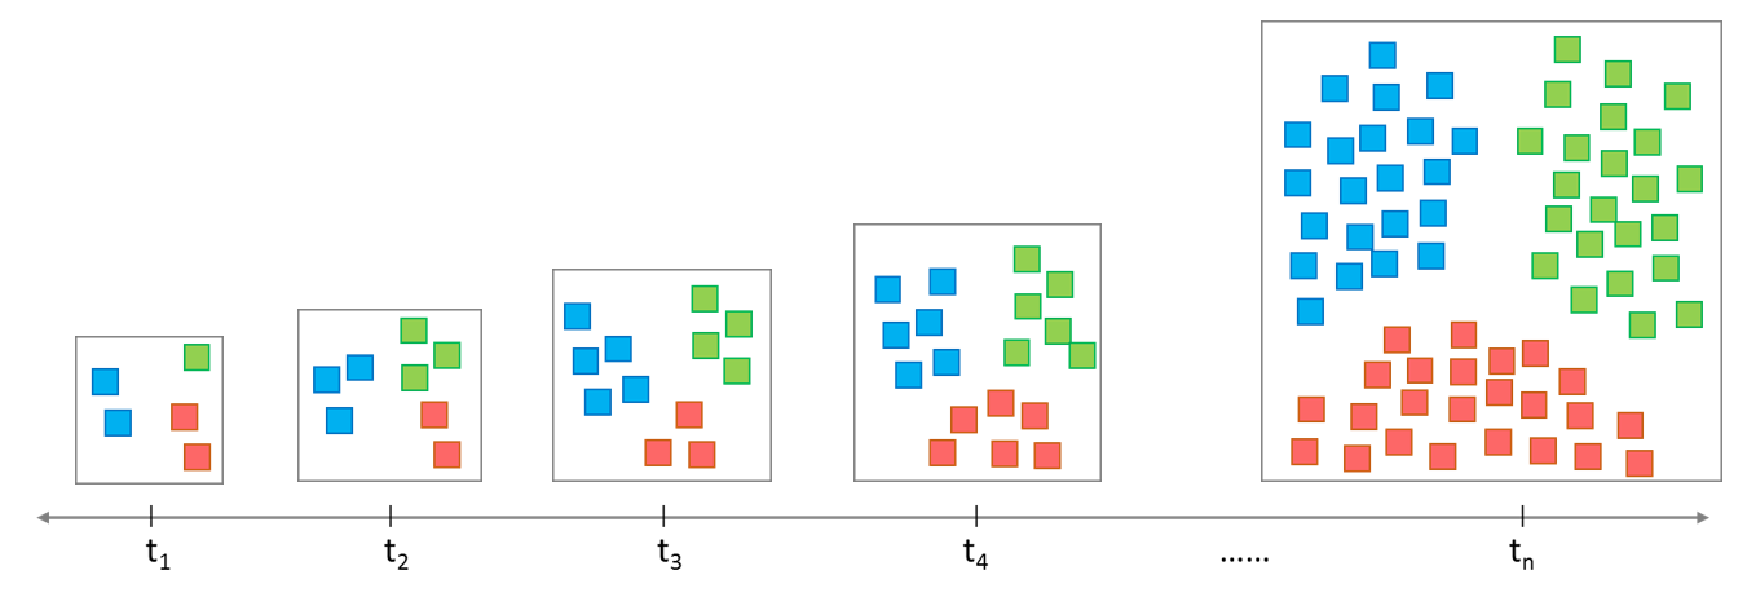
\includegraphics[width=\textwidth]{Figures/Introduction/Fig4.pdf}
    \caption{Training with Batch Methods}
  \end{subfigure}
  
  \begin{subfigure}[h]{0.75\textwidth}
	\centering
    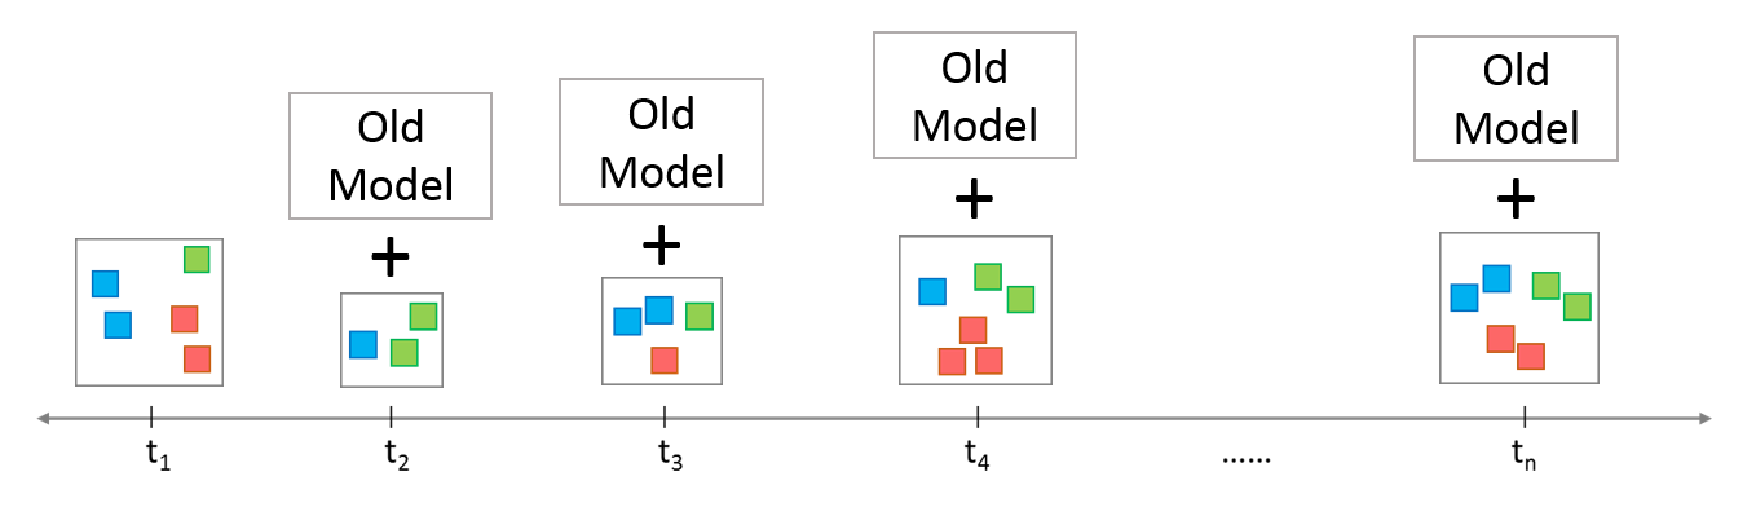
\includegraphics[width=\textwidth]{Figures/Introduction/Fig5.pdf}
    \caption{Training with Incremental Methods}
  \end{subfigure}
\caption{Batch methods vs. Incremental methods: (a) Batch methods have to retrain on all the historical data after every addition. (b) Incremental methods only need the old model and new data samples to update the model after every addition.}
\label{fig:Intro_Inc}
\end{figure}


The increment in single-view data may occur in two types-first adds one data sample at a time, termed as \textit{sequential increment} and the other adds a group of data samples at a time, termed as \textit{chunk increment}. The number of data samples added in one increment may or may not be the same as that in the previous increment. Incremental methods for single-view data include methods based on LDA \cite{PangOK05, KumarM21}, PCA \cite{ZhaoYK06, LiuCZ18} as well as SVM \cite{GuQGSZ18}. Some of the extensions \cite{CauwenberghsP00, ChenXXZ19, LeeKWLL19, Kashef21} of SVM are presented as incremental-decremental methods that allow addition as well as deletion of data samples. However, when used on multi-view data, the single-view methods treat all the views as one and lose the discriminating information each view offers. Hence, these methods are not equipped to handle multi-view data.

In the multi-view context, the increment can be of two types - the first is \textit{data sample increment}, where the number of data samples gets updated with time, but the number of views remains unchanged. The new data samples are added to all the existing views simultaneously. We see the applications of this type of increment in tasks such as video surveillance \cite{LopezRPFL19} and autonomous driving \cite{OliveiraSSDM16} where new training samples are added from all the cameras or other sensors. The other type of increment is \textit{view increment}, where the number of data samples is fixed, and the number of views is updated over time as new views of every existing data sample are added. This type of increment is seen when information from sensors, cameras, or other information capture tools that were previously not included is added to gather new views of data in the recognition or detection systems mentioned above.
% To continue the previous example, let us assume we have view-1 and view-2 of twelve fruit samples and a model trained on this data. Now, if we wish to add another instance of an `apple', we must add its feature information in both the views, i.e., shape- \textit{heart-shaped} and color- \textit{red}. Each view now has thirteen data samples. 
% In the example above, view-1 and view-2 of data have thirteen data samples each. We add a third view of \textit{cross-section} of all thirteen fruits to this dataset. Here, we do not include new fruits. We only include a new view of the existing fruits.

The incremental learning paradigm is still in its early stages of development. Most of the works report the advantages and the results of these methods. Due to the lack of comparative or analytical studies, the challenges faced by the incremental methods have not been studied extensively. Nevertheless, we find two major challenges listed in the literature- First is termed as \textit{catastrophic forgetting} which refers to the situation where the learning algorithm forgets the older data while learning from the new samples. The other challenge is the \textit{order of update}, where the order of addition or deletion of data samples changes the learned model considerably. Discriminant analysis-based methods do not face these problems as the scatter matrices are computed by adding the scatter of each data sample together, leading to the ability to remember all data samples and order-invariance. Another challenge is faced by the methods that retain some of the older data samples. These methods must devise a strategy to select the data samples that are most informative as there is often an imposition on the number of data samples a model can retain in their original form.

In real life, we see many applications that are of incremental nature and use newer data to produce up-to-date results. One such system to use incremental learning is an autonomous driving system \cite{OliveiraSSDM16} that collects data and incrementally learns to recognize different objects from every new encounter. Though many incremental learners keep expanding their knowledge-base by learning new information, others may choose to forget some of the older data samples for better performance. For example, the recommendation engine \cite{ZhangYC19} of the online video platforms collects the watch history and recommends more videos related to the latest favorites of the user. Here, the system may choose to forget some or all of older data as it has become obsolete due to the changed preferences of the user.






\subsubsection*{2D Learning}
\label{ssubs:Intro_2D}
2D learning is designed for image-based datasets and is about changing the use of data for training. Traditionally, useful features from these images are extracted to train on image-based data for various computer vision tasks. Such features are often one-dimensional and specialize in capturing a particular aspect of the image, such as histograms, corners, or blobs. If the features are 2D, they must be reshaped into 1D vectors before training.

While these features are useful, they have some disadvantages. The first disadvantage is the one-dimensional nature of such features. These features, being one-dimensional, are less suitable for capturing the structural or spatial information that is better stored in a 2D image matrix. Hence, the vectorization defeats the purpose of having 2D data or 2D features. Secondly, these specialized features may not carry all the information that is valuable to the learning task. One has to use a combination of many features to gather the required information from an image. Lastly, as the size of one-dimensional features is often large, we have to face the problem of singularity. For example, if the size of the images in a dataset is $p \times q$, then the size of the feature vector will be $pq$. If one wishes to use these features, the size of the scatter matrix will be $pq \times pq$, which is very large compared to the small number of data samples in a typical image processing dataset. This issue becomes even more prominent with the emergence of new technology, as high-definition images lead to even larger feature vectors.

To address these issues of 1D methods, one can directly use the original image matrix. The original matrix form stores the spatial information better as it is inherently two-dimensional. The original 2D image has all the information within itself, so we do not need to extract any other features. It also tackles the singularity issue as the number of dimensions of the scatter matrix is significantly less than that when computed with the one-dimensional features. Continuing with the example above, when the matrix form of an image of size $r \times c$ is used directly, the size of the scatter matrix will be $r \times r$ instead of $rc \times rc$. Fig. \ref{fig:Intro_2D} shows how the use of 2D data in its original form produces a smaller scatter matrix than the 1D data. Another benefit of 2D data is that its use eliminates the efforts put into feature extraction. These qualities of original 2D image data make it a better candidate for training a classification model. To use it for training, we need methods designed for the 2D data.


\begin{figure}[t]
\centering
	\begin{subfigure}[t]{0.45\textwidth}
		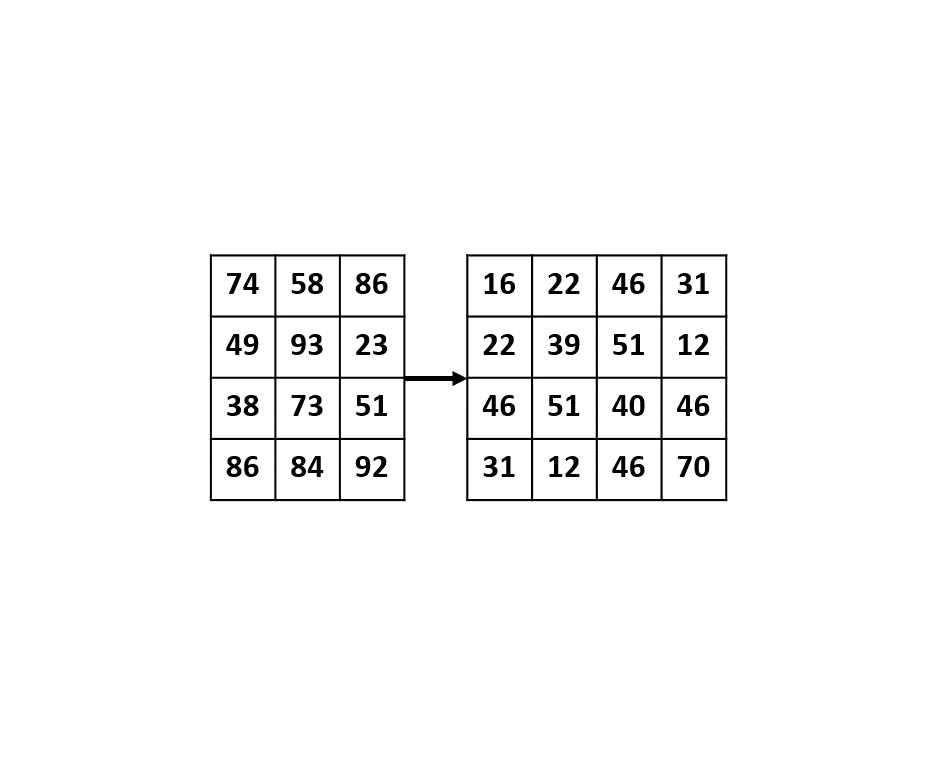
\includegraphics[width=\textwidth]{Figures/Introduction/Fig6.png}
		\caption{Scatter matrix using 2D data}
		\label{fig:Intro_2D_2D}
	\end{subfigure}\hspace{0.2cm}
	\begin{subfigure}[t]{0.45\textwidth}
		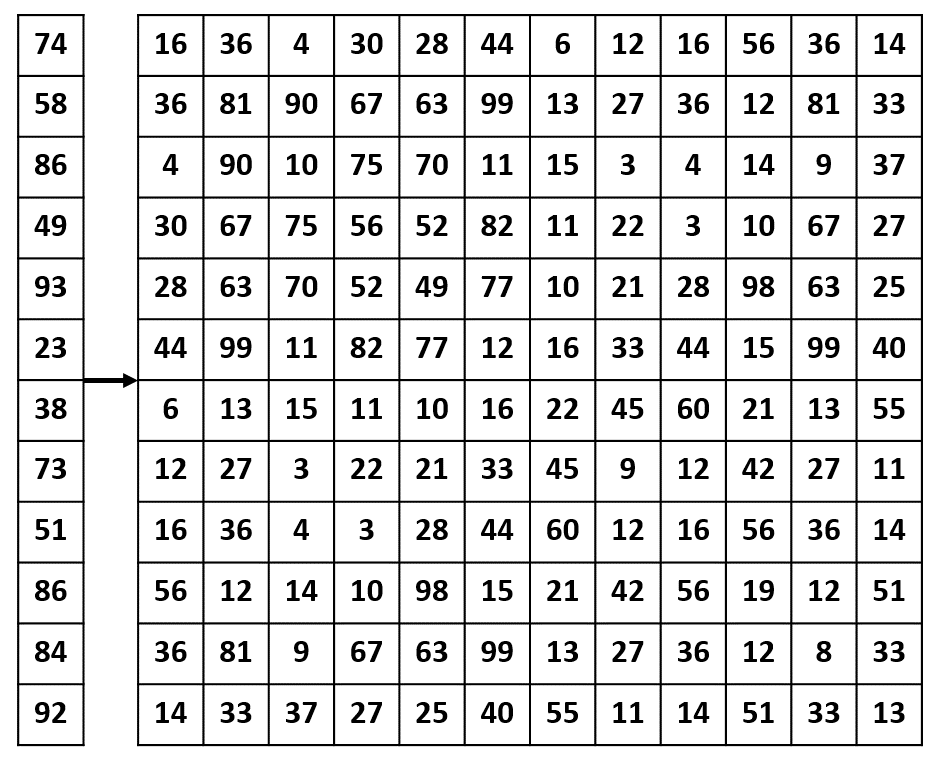
\includegraphics[width=\textwidth]{Figures/Introduction/Fig7.png}
		\caption{Scatter matrix using 1D data}
		\label{fig:Intro_2D_1D}
	\end{subfigure}
	\caption{Difference between the sizes of scatter matrices- (a) 2D data of size $4 \times 3$ produces a scatter matrix of size $4 \times 4$. (b) The vectorized form of the same input matrix produces scatter matrix of size $12 \times 12$.}
	\label{fig:Intro_2D}
\end{figure}


2D methods are fairly restricted in terms of the domains where they can be used. However, their impact cannot be ignored. Natural 2D data is used primarily in computer vision and image processing applications. Though conceptualized as early as in 1991 \cite{TurkP91}, these methods are just now finding their footing in the literature. 2D methods play a significant role for tasks such as face \cite{ZhangDNLZG19}, gait \cite{WuSZ19}, and character \cite{CaiW18} recognition, among others. However, these are all single-view methods, and the multi-view paradigm has not yet benefited from the advantages these methods offer. The main goal of using 2D data is to reduce computational memory. Hence, methods that deal with multi-view data that can be very large will benefit from 2D methods.











\section{Contributions of the Thesis}
\label{sec:Intro_Contributions}
\begin{figure}[t]
	\centering
	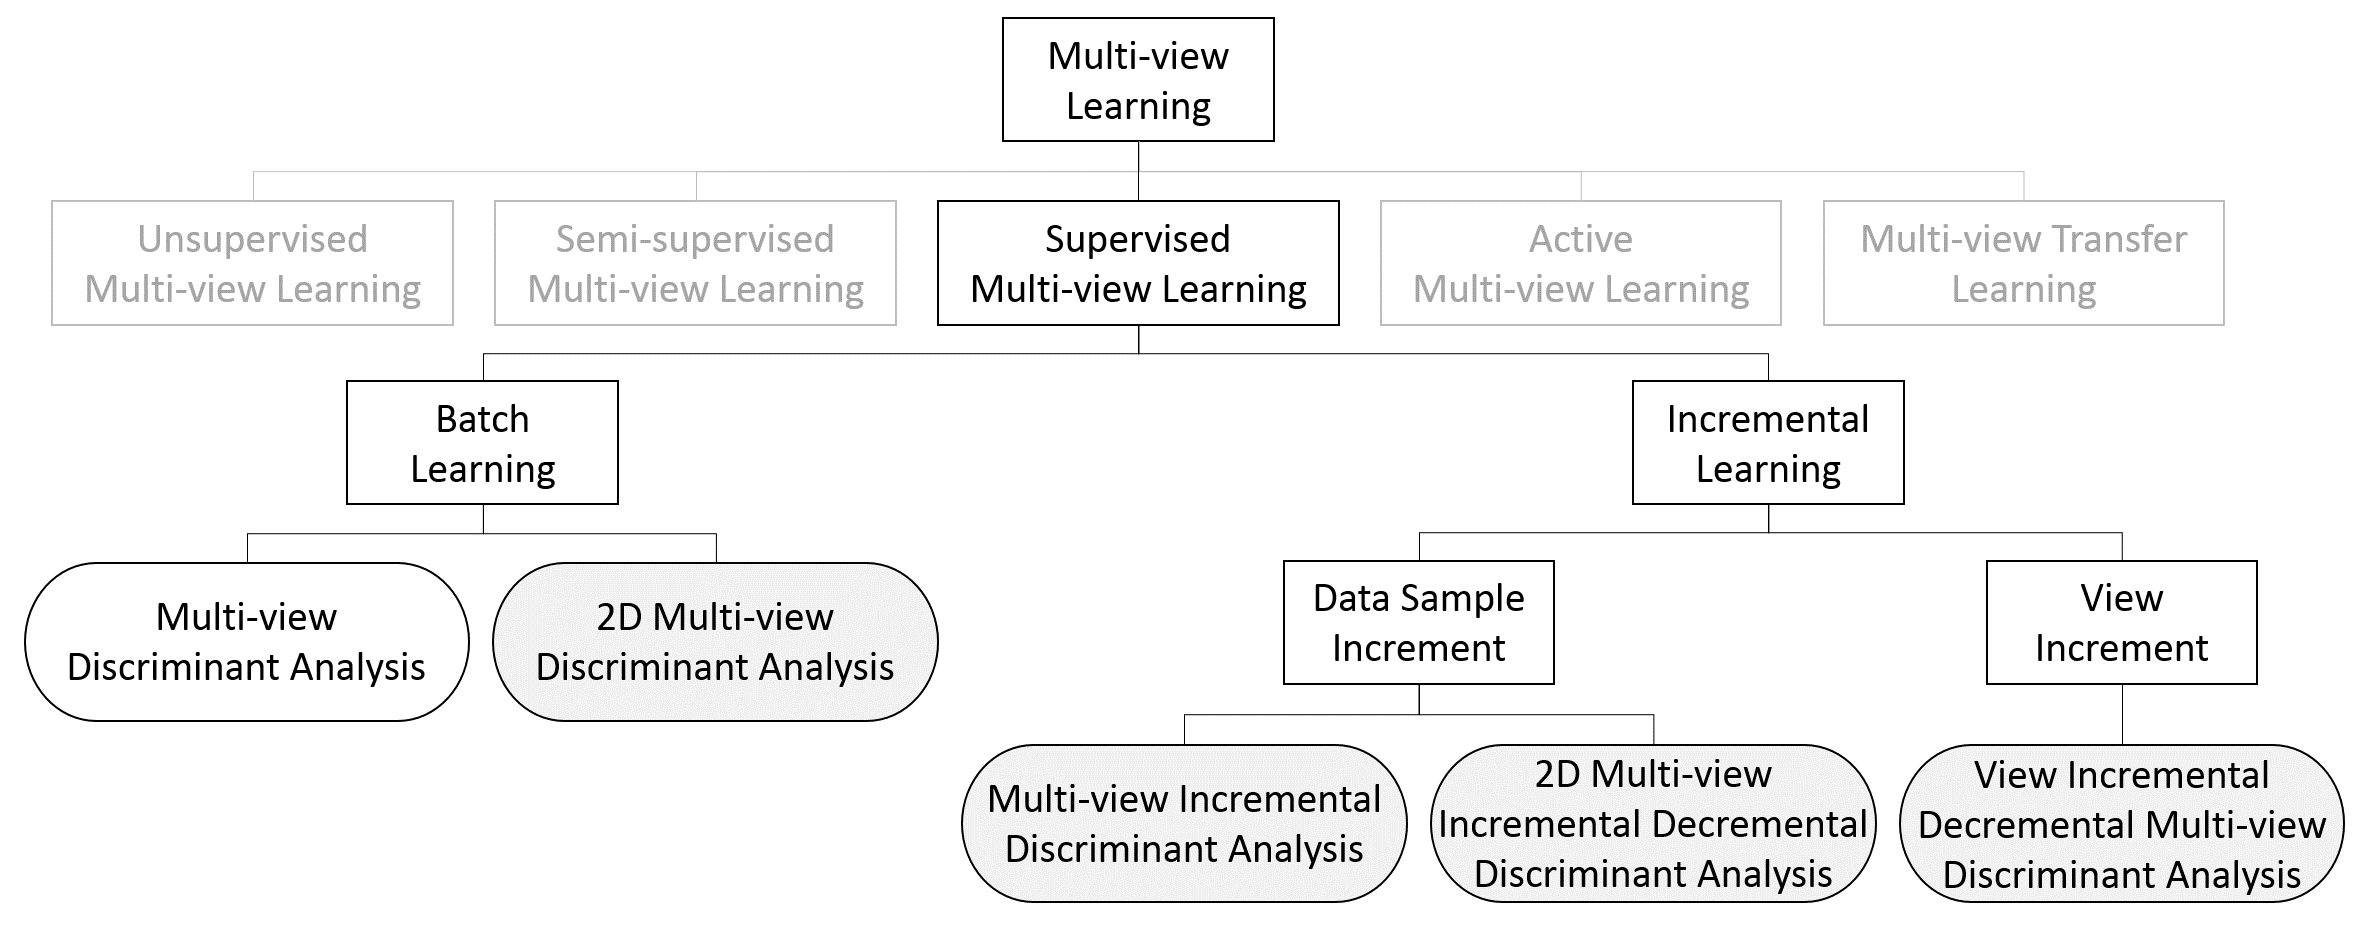
\includegraphics[width=\textwidth]{Figures/Introduction/Fig8.png}
	\caption{The placement of presented methods in the multi-view learning paradigm.}
	\label{fig:Intro_Methods}
\end{figure}


In this thesis, we present four methods that fill four niches in multi-view learning. We introduce incremental learning to the multi-view domain with our first method that supports the inclusion of new data samples. Then, we formulate a multi-view batch learning method for 2D data. This method is then extended to support incremental learning and decremental unlearning of data samples in the 2D multi-view domain in the third method. Lastly, we present a method to incrementally learn or decrementally unlearn the views of data. All of these methods belong to the supervised learning domain and are based on Multi-view Discriminant Analysis (MvDA) \cite{KanSZLC16}. These methods use incremental learning and 2D learning paradigms to achieve their goals. Fig. \ref{fig:Intro_Methods} shows where the presented methods stand in the multi-view learning paradigm.


\subsection{Contribution 1: An Incremental Method for 1D Multi-view Data}
Multi-view batch methods have proved their utility by producing better results than single-view methods. However, when working with incremental data, these methods need to retrain from scratch after every addition in the dataset. We need incremental methods for training efficiently on the incremental data. The following research questions are investigated in this regard.



\begin{description}
\item[\textbf{RQ1: }] \textbf{Can an incremental method, without using old data samples, produce an identical model to that of its batch counterpart MvDA?}

\item[\textbf{RQ2: }] \textbf{Is this incremental method invariant to the order of addition of new data samples?}

\item[\textbf{RQ3: }] \textbf{Can this incremental method reduce training time?}

\item[\textbf{RQ4: }] \textbf{Can this incremental method reduce memory requirements?}

\item[\textbf{RQ5: }] \textbf{Is this multi-view incremental method more advantageous than a single-view incremental method in terms of classification accuracy and training time?}

\item[\textbf{Solution: }] We present Multi-view Incremental Discriminant Analysis (MvIDA), which supports the addition of new data samples without using the old data samples. MvIDA offers a closed-form solution to update the existing model using only the new data samples. It considers all the views and jointly solves the linear transform to find the same optimal common discriminant space as a batch method.

\item[\textbf{Results:}] The experiments carried out on three 1D multi-view datasets show that the proposed method indeed finds the same subspace as its batch counterpart. Moreover, the produced model does not depend on the order or the number of data samples in each increment. MvIDA is also shown to perform the updates in less time and memory than MvDA due to its incremental nature. Incremental Linear Discriminant Analysis (ILDA) is a single-view incremental method based on discriminant analysis. The comparison of MvIDA with ILDA shows that using a multi-view incremental method on multi-view data produces better results than those obtained using a single-view incremental method. This comparison also shows that MvIDA requires less training time than ILDA.
\end{description}



\subsection{Contribution 2: A Batch Method for 2D Multi-view Data}
Image-based data is best represented in its original 2D form, as this form preserves spatial information. However, due to the lack of methods that support the use of 2D multi-view data, it must be converted in the vectorized form before it is used for training. To tackle this, we need improved multi-view methods that can train on the 2D form eliminating the need for vectorization. The following research questions are investigated in order to fulfill this need.


\begin{description}
\item[\textbf{RQ1: }] \textbf{Can a 2D multi-view method build better classification model than a 1D multi-view method or a 2D single-view method?}

\item[\textbf{RQ2: }] \textbf{Can the use of 2D matrices reduce training time?}

\item[\textbf{RQ3: }] \textbf{Can the use of 2D matrices reduce memory requirements?}

\item[\textbf{Solution:}] We present 2D Multi-view Discriminant Analysis (2DMvDA), which can use the 2D multi-view data without having to vectorize it before training. Like MvIDA, this method also solves the linear transforms of every view together and forms an optimal common discriminant subspace. This method also forms the basis for its incremental version presented in the following contribution.

\item[\textbf{Results:}] The experiments carried out on four 2D datasets show that the proposed method benefits from the direct use of 2D data in two ways: (i) it generates significantly smaller scatter matrices, leading to reduced time and memory costs. (ii) it preserves spatial information, leading to improved classification accuracy. The comparison of training time and memory requirements shows that the proposed method needs less time and memory than the 1D multi-view method (MvDA) and a 2D single-view method (2DLDA).
\end{description}



\subsection{Contribution 3: An Incremental Decremental Method for 2D Multi-view Data}
Though MvIDA has been proposed for multi-view incremental data, it does not support 2D data. Moreover, it only supports the addition of the data samples. For 2D incremental data, we need a method that can train on the original matrix form of the data. Also, to facilitate the removal of the obsolete data samples from the model, we need a method that supports decremental unlearning.


\begin{description}
\item[\textbf{RQ1: }] \textbf{Can the 2D incremental-decremental method, without using old data samples, produce an identical model to that of its batch counterpart, 2DMvDA?}

\item[\textbf{RQ2: }] \textbf{Is this method invariant to the order of addition or deletion of data samples?}

\item[\textbf{RQ3: }] \textbf{Is this method more advantageous than other discriminant analysis-based methods?}

\item[\textbf{Solution:}] We present a method, 2D Multi-view Incremental Decremental Discriminant Analysis (2DMvIDDA), which supports the addition and deletion of data samples at any point in time. It provides closed-form solutions to update the scatter matrices without retraining after each addition/deletion. This method can also be transformed into other methods based on discriminant analysis, such as MvIDA, 2DMvDA, MvDA, 2DLDA, and ILDA, with minor changes to the formulation.

\item[\textbf{Results:}] The experiments show that 2DMvIDDA produces the same discriminant subspace as its batch counterpart 2DMvDA and is order-independent. The experiments to compare 2DMvIDDA with other methods based on discriminant analysis are carried out in two parts. The first set compares these methods on rescaled versions of four 2D datasets to show that 2DMvIDDA attains the best classification accuracy among all these methods using considerably less time and memory owing to its use of all three paradigms. The rescaled versions are used here because the 1D methods could not train on the original datasets due to their huge memory requirements. The second set of experiments trains the model using only the 2D methods- 2DMvIDDA, 2DMvDA, and 2DLDA on the original versions of the same four datasets to show the vast difference in memory requirements of 1D vs. 2D methods.
\end{description}



\subsection{Contribution 4: A View Incremental Decremental Method for Multi-view Data}
Increment/decrement in multi-view context is of two types: data sample increment and view increment. MvIDA and 2DMvIDDA belong to the \textit{data sample increment} category. However, to support the addition or deletion of views of data, we need a view incremental method.


\begin{description}
\item[\textbf{RQ1: }] \textbf{Can the incremental-decremental method, without using old views, produce an identical model to that of its batch counterpart MvDA?}

\item[\textbf{RQ2: }] \textbf{Is this method invariant to the order of addition or deletion of data samples?}

\item[\textbf{RQ3: }] \textbf{Can this method perform as well as the batch method in terms of classification accuracy?}

\item[\textbf{RQ4: }] \textbf{Can this method reduce training time?}

\item[\textbf{RQ5: }] \textbf{Can this method reduce memory requirements?}

\item[\textbf{Solution:}] We present View Incremental Decremental Multi-view Discriminant Analysis (VIDMvDA), which supports incremental learning and decremental unlearning of the views of data without retraining. VIDMvDA jointly solves multiple linear transforms to produce the same optimal common discriminant subspace as its batch counterpart MvDA. Though presented for 1D data, VIDMvDA can also be used as a 2D method.

\item[\textbf{Results:}] The experiments on three 1D datasets show that the proposed method finds the same or sometimes better common subspace than its batch counterpart, MvDA. It is proven to be order-independent and has the same or slightly better classification accuracy than MvDA. VIDMvDA also updates the model to include or exclude the views using less time and memory than MvDA.
\end{description}











\section{Organization of the Thesis}
\label{sec:Organization}
The thesis is comprised of eight chapters. The chapter-wise organization of the thesis is given below: 

\begin{description}
	
	\item[Chapter 2] reviews multi-view batch methods and single-view incremental methods. It also takes a look at the methods that emerged out of a combination of multi-view and incremental learning, namely data-incremental and view-incremental multi-view methods. We then present single-view batch methods for 2D data, as 2D learning is a relatively new paradigm and does not have any multi-view or incremental methods. In this chapter, we also briefly go through the workings of a recent multi-view batch method, Multi-view Discriminant Analysis (MvDA), which serves as an inspiration for our methods presented in this thesis. MvDA is, as the name suggests, based on discriminant analysis.
	
	\item[Chapter 3] introduces the terminology and notations used by the methods in this thesis and states the assumptions made by these methods. Then, it describes the 1D and 2D datasets used for experiments that measure the performance of presented methods.
	
	\item[Chapter 4] presents the formulations of our first contribution, Multi-view Incremental Discriminant Analysis (MvIDA), and the experimental results thereof. MvIDA is an incremental classification method based on discriminant analysis for multi-view data.
	
	\item[Chapter 5] presents a classification method for 2D multi-view data. This batch method, 2D Multi-view Discriminant Analysis (2DMvDA), serves as a basis to introduce an incremental method in the context of 2D multi-view data in chapter \ref{ch:2DMvIDDA}.
	
	\item[Chapter 6] presents 2D Incremental Decremental Discriminant Analysis (2DMvIDDA), an incremental-decremental classification method for 2D multi-view data. This method can be converted into MvDA, ILDA, 2DLDA, MvIDA, and 2DMvDA.
	
	\item[Chapter 7] presents an incremental-decremental method that supports view-wise addition or deletion. This method, View Incremental Decremental Multi-view Discriminant Analysis (VIDMvDA), incrementally learns or decrementally unlearns the views of data. 
	
	\item[Chapter 8] highlights the conclusions and summarizes the contributions made. New avenues for future research have also been discussed.
	
\end{description}

\chapterend